\documentclass[12pt,a4paper,UTF8]{article}
\usepackage{ctex}               % 中文支持
\usepackage{amsmath,amssymb}   % 数学公式
\usepackage{graphicx}          % 图片
\setkeys{Gin}{width=0.85\textwidth} % 统一所有图片宽度（防止溢出）
\usepackage{geometry}          % 页边距
\usepackage{fancyhdr}          % 页眉页脚
\usepackage{tikz}              % 绘制根轨迹图
\usetikzlibrary{arrows.meta}   % 箭头样式

% 页边距设置
\geometry{left=2.5cm,right=2.5cm,top=2.5cm,bottom=2.5cm}

% 页眉页脚
\pagestyle{fancy}
\fancyhf{}
\cfoot{\thepage}

% 公式、图表、段落优化
\linespread{1.2}
\parindent 2em

\begin{document}

\begin{titlepage}
    \centering
    \vspace*{5cm}
    \Huge\bfseries 拉普拉斯变换作业
    \vspace*{\fill}
\end{titlepage}
\newpage
\input{3.绪论.tex}
\section{拉普拉斯变换计算题}

\subsection{题目1}
求函数 $f(t) = 5e^{-2t} - \sin 2t,\ t \geq 0$ 的Laplace变换。

\subsubsection{解答}
根据拉普拉斯变换的线性性质，分别对两项进行变换：
\begin{align*}
    \mathcal{L}\left[5e^{-2t}\right] &= 5 \cdot \mathcal{L}\left[e^{-2t}\right] = 5 \cdot \frac{1}{s+2}, \quad (\text{指数函数变换公式：}\mathcal{L}[e^{-at}] = \frac{1}{s+a}) \\
    \mathcal{L}\left[\sin 2t\right] &= \frac{2}{s^2 + 2^2} = \frac{2}{s^2 + 4}, \quad (\text{正弦函数变换公式：}\mathcal{L}[\sin \omega t] = \frac{\omega}{s^2+\omega^2})
\end{align*}
因此，原函数的拉普拉斯变换为：
\begin{align*}
    F(s) &= \mathcal{L}\left[5e^{-2t} - \sin 2t\right] \\
    &= 5\mathcal{L}\left[e^{-2t}\right] - \mathcal{L}\left[\sin 2t\right] \\
    &= \frac{5}{s+2} - \frac{2}{s^2+4} \\
    &= \frac{5(s^2+4) - 2(s+2)}{(s+2)(s^2+4)} \\
    &= \frac{5s^2 - 2s + 16}{s^3 + 2s^2 + 4s + 8}
\end{align*}
最终结果：
\[
\boxed{F(s) = \frac{5}{s+2} - \frac{2}{s^2+4} = \frac{5s^2 - 2s + 16}{s^3 + 2s^2 + 4s + 8}}
\]

\newpage
\subsection{题目2}
求函数 $F(s) = \dfrac{2s+2}{s^2+2s+5}$ 的Laplace逆变换。

\subsubsection{解答}
首先对分母进行配方，将其化为标准形式：
\[
s^2 + 2s + 5 = (s+1)^2 + 2^2
\]
对分子进行拆分，匹配标准逆变换形式：
\[
2s+2 = 2(s+1)
\]
因此原函数可改写为：
\[
F(s) = \frac{2(s+1)}{(s+1)^2 + 2^2}
\]
根据拉普拉斯逆变换的频移性质：
\[
\mathcal{L}^{-1}\left[\frac{s+a}{(s+a)^2 + \omega^2}\right] = e^{-at}\cos\omega t
\]
代入 $a=1,\ \omega=2$，可得：
\begin{align*}
    f(t) &= \mathcal{L}^{-1}\left[\frac{2(s+1)}{(s+1)^2 + 2^2}\right] \\
    &= 2 \cdot \mathcal{L}^{-1}\left[\frac{s+1}{(s+1)^2 + 2^2}\right] \\
    &= 2e^{-t}\cos 2t,\quad t \geq 0
\end{align*}
最终结果：
\[
\boxed{f(t) = 2e^{-t}\cos 2t,\ t \geq 0}
\]
\input{5.控制系统的时域分析.tex}
\section{线性系统的根轨迹法}
本节针对5道典型习题，依次完成根轨迹绘制、特征参数计算、系统稳定性与动态性能分析，所有推导过程规范完整。

\subsection{6.1 常规根轨迹绘制}
某反馈系统的开环传递函数为：
\[
G(s)H(s)=\frac{K'(s+0.1)(0.6s+1)}{s^2(s+0.01)}
\]
试绘制增益 $K$ 从 $0$ 到 $\infty$ 时系统的闭环根轨迹。

\subsubsection{解题步骤与推导}
将开环传递函数化为标准根轨迹形式：
\[
G(s)H(s) = \frac{K(s+0.1)(s+1.67)}{s^2(s+0.01)},\quad K=0.6K'
\]

\begin{enumerate}
    \item \textbf{开环零极点}：
    极点 $p_1=p_2=0,\ p_3=-0.01$；零点 $z_1=-0.1,\ z_2=-1.67$。

    \item \textbf{根轨迹分支数}：$n=3$，共3支。

    \item \textbf{实轴上的根轨迹}：
    $(-\infty,-1.67],\ [-0.1,-0.01]$。

    \item \textbf{渐近线}：
    $n-m=1$，渐近线角度 $\varphi_a=180^\circ$，
    与实轴交点 $\sigma_a=1.76$。

    \item \textbf{分离点与会合点}：
    由 $\dfrac{\mathrm{d}}{\mathrm{d}s}\left[\ln(G(s)H(s))\right] = 0$ 求解。

    \item \textbf{虚轴交点}：
    代入 $s=j\omega$，由特征方程 $1+G(s)H(s)=0$ 求解。
\end{enumerate}

\begin{center}
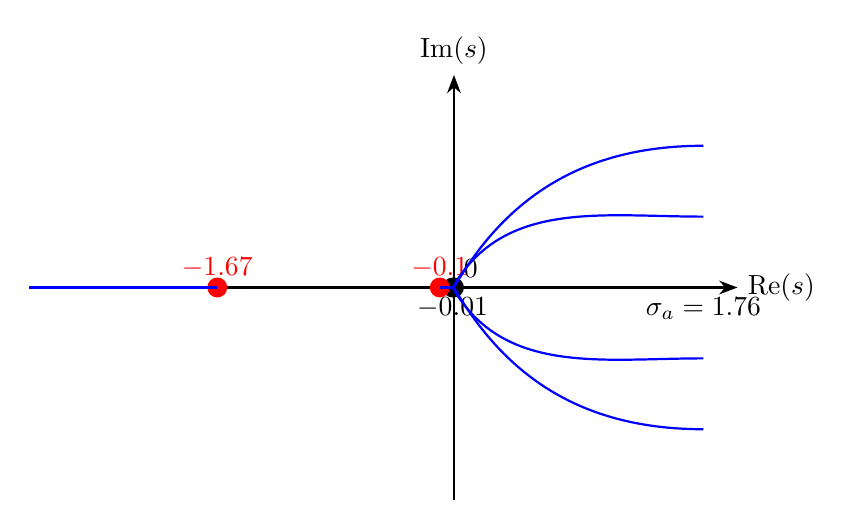
\begin{tikzpicture}[scale=1.8, >=Stealth]
\draw[->, thick] (-3,0) -- (2,0) node[right] {$\mathrm{Re}(s)$};
\draw[->, thick] (0,-1.5) -- (0,1.5) node[above] {$\mathrm{Im}(s)$};

% 极点
\fill (0,0) circle (2pt) node[above right] {$0$};
\fill (-0.01,0) circle (2pt) node[below] {$-0.01$};

% 零点
\fill[red] (-0.1,0) circle (2pt) node[above] {$-0.1$};
\fill[red] (-1.67,0) circle (2pt) node[above] {$-1.67$};

% 根轨迹
\draw[thick, blue] (-3,0) -- (-1.67,0);
\draw[thick, blue] (-0.1,0) -- (-0.01,0);
\draw[thick, blue] (0,0) to[out=60,in=180] (1.76,1);
\draw[thick, blue] (0,0) to[out=-60,in=180] (1.76,-1);
\draw[thick, blue] (-0.01,0) to[out=60,in=180] (1.76,0.5);
\draw[thick, blue] (-0.01,0) to[out=-60,in=180] (1.76,-0.5);

\node at (1.76,0) [below] {$\sigma_a=1.76$};
\end{tikzpicture}

\small 图6.1 系统根轨迹图
\end{center}

\newpage
\subsection{6.2 二阶系统根轨迹与动态性能分析}
已知单位负反馈系统开环传递函数
\[
G(s)=\frac{K(s+2)}{s(s+1)}
\]
试完成：
\begin{enumerate}
    \item 绘制根轨迹
    \item 求 $\zeta=\dfrac{\sqrt{2}}{2}$ 时的增益 $K$
    \item 求系统欠阻尼增益范围
\end{enumerate}

\subsubsection{解题步骤与推导}
\begin{enumerate}
    \item \textbf{根轨迹绘制}
    极点：$0,\ -1$；零点：$-2$。
    实轴根轨迹：$(-\infty,-2],\ [-1,0]$。
    渐近线：$n-m=1$，$\varphi_a=180^\circ$。
    根轨迹为圆心 $(-2,0)$、半径 $\sqrt{2}$ 的圆。

    \item \textbf{当 $\zeta=\dfrac{\sqrt{2}}{2}$ 时}
    阻尼角 $\theta=45^\circ$，特征根为
    \[
    s_{1,2}=-1\pm j1
    \]
    代入幅值条件得 $K=1$。

    \item \textbf{欠阻尼范围}
    分离点 $d=-0.586$，对应 $K=0.172$，
    故欠阻尼范围为
    \[
    K>0.172
    \]
\end{enumerate}

最终结论：
\[
\boxed{K=1},\quad \boxed{s_{1,2}=-1\pm j1},\quad \boxed{K>0.172}
\]

\begin{center}
\begin{tikzpicture}[scale=1.8, >=Stealth]
\draw[->, thick] (-4,0) -- (1,0) node[right] {$\mathrm{Re}(s)$};
\draw[->, thick] (0,-2) -- (0,2) node[above] {$\mathrm{Im}(s)$};

% 极点
\fill (0,0) circle (2pt) node[above right] {$0$};
\fill (-1,0) circle (2pt) node[below] {$-1$};

% 零点
\fill[red] (-2,0) circle (2pt) node[above] {$-2$};

% 根轨迹圆
\draw[thick, blue] (-2,0) circle (1.414);
\draw[thick, blue] (-4,0) -- (-2,0);
\draw[thick, blue] (-1,0) -- (0,0);

% 特征点
\fill (-1,1) circle (2pt) node[above right] {$-1+j1$};
\fill (-1,-1) circle (2pt) node[below right] {$-1-j1$};
\draw[dashed, gray] (-1,1) -- (0,0);
\node at (-0.5,0.3) {$45^\circ$};
\end{tikzpicture}

\small 图6.2 系统根轨迹图
\end{center}

\newpage
\subsection{6.3 四重极点系统根轨迹与稳定性分析}
已知开环传递函数
\[
G(s)=\frac{K}{(s+1)^2(s+4)^2}
\]
绘制根轨迹并求稳定范围。

\subsubsection{解题步骤与推导}
\begin{enumerate}
    \item \textbf{零极点}：
    二重极点 $-1$、$-4$；无零点。

    \item \textbf{渐近线}：
    角度 $\pm45^\circ,\pm135^\circ$，交点 $\sigma_a=-2.5$。

    \item \textbf{分离点}：$d=-2.5$。

    \item \textbf{虚轴交点}：
    由劳斯判据得临界增益 $K=100$。

    \item \textbf{稳定范围}：
    \[
    0<K<100
    \]
\end{enumerate}

\begin{center}
\begin{tikzpicture}[scale=1.2, >=Stealth]
\draw[->, thick] (-6,0) -- (2,0) node[right] {$\mathrm{Re}(s)$};
\draw[->, thick] (0,-4) -- (0,4) node[above] {$\mathrm{Im}(s)$};

% 极点
\fill (-1,0) circle (2pt) node[above] {$-1$ (二重)};
\fill (-4,0) circle (2pt) node[above] {$-4$ (二重)};

% 渐近线
\draw[dashed, gray] (-2.5,0) -- (-2.5,3);
\draw[dashed, gray] (-2.5,0) -- (-2.5,-3);
\draw[dashed, gray] (-2.5,0) -- (0,2.5);
\draw[dashed, gray] (-2.5,0) -- (0,-2.5);

% 根轨迹
\draw[thick, blue] (-6,0) -- (-4,0);
\draw[thick, blue] (-1,0) to[out=135,in=45] (-2.5,2);
\draw[thick, blue] (-1,0) to[out=-135,in=-45] (-2.5,-2);
\draw[thick, blue] (-4,0) to[out=45,in=135] (-2.5,2);
\draw[thick, blue] (-4,0) to[out=-45,in=-135] (-2.5,-2);

\node at (-2.5,0) [below] {$\sigma_a=-2.5$};
\end{tikzpicture}

\small 图6.3 系统根轨迹图
\end{center}

\newpage
\subsection{6.4 零度根轨迹绘制与收敛性能分析}
已知开环传递函数
\[
G(s)=\frac{K^*(1-s)}{(s+1)(s+2)}
\]
绘制零度根轨迹并求振荡收敛增益范围。

\subsubsection{解题步骤与推导}
化为标准形式：
\[
G(s)=\frac{-K^*(s-1)}{(s+1)(s+2)}
\]
属于**正反馈根轨迹（零度根轨迹）**。

\begin{enumerate}
    \item 极点：$-1,-2$；零点：$1$。
    \item 实轴根轨迹：$[-2,-1],\ [1,+\infty)$。
    \item 渐近线角度：$0^\circ$。
    \item 分离点：$d=-1.5$。
    \item 收敛（欠阻尼）范围：
    \[
    2<K^*<6
    \]
\end{enumerate}

\begin{center}
\begin{tikzpicture}[scale=1.8, >=Stealth]
\draw[->, thick] (-3,0) -- (3,0) node[right] {$\mathrm{Re}(s)$};
\draw[->, thick] (0,-2) -- (0,2) node[above] {$\mathrm{Im}(s)$};

% 极点
\fill (-1,0) circle (2pt) node[below] {$-1$};
\fill (-2,0) circle (2pt) node[below] {$-2$};

% 零点
\fill[red] (1,0) circle (2pt) node[above] {$1$};

% 根轨迹
\draw[thick, blue] (-2,0) -- (-1,0);
\draw[thick, blue] (1,0) -- (3,0);
\draw[thick, blue] (-1.5,0) to[out=60,in=180] (0,1);
\draw[thick, blue] (-1.5,0) to[out=-60,in=180] (0,-1);
\draw[thick, blue] (1,0) to[out=120,in=0] (0,1);
\draw[thick, blue] (1,0) to[out=-120,in=0] (0,-1);

\node at (-1.5,0) [below] {$-1.5$};
\end{tikzpicture}

\small 图6.4 零度根轨迹图
\end{center}

\newpage
\subsection{6.5 参变量根轨迹与实轴交点分析}
系统特征方程：
\[
s^2(s+a)+k(s+1)=0
\]
以 $k$ 为参变量，分析根轨迹与负实轴交点情况。

\subsubsection{解题步骤与推导}
化为根轨迹方程：
\[
1+\frac{k(s+1)}{s^2(s+a)}=0
\]
分离点方程：
\[
s^2+(3+a)s+2a=0
\]
判别式：
\[
\Delta=(a-1)^2+8>0
\]
故**始终有两个分离点**。

结论：
\begin{enumerate}
    \item $a>0$：两个负实轴分离点；
    \item $a=0$：一个负实轴分离点；
    \item $a<0$：无负实轴分离点。
\end{enumerate}

最终结论：
\[
\boxed{
\begin{aligned}
&a>0 \text{ 时，根轨迹与负实轴有两个交点；} \\
&a=0 \text{ 时，有一个交点；} \\
&a<0 \text{ 时，无交点。}
\end{aligned}
}
\]

\begin{center}
\begin{tikzpicture}[scale=1.8, >=Stealth]
\draw[->, thick] (-4,0) -- (1,0) node[right] {$\mathrm{Re}(s)$};
\draw[->, thick] (0,-2) -- (0,2) node[above] {$\mathrm{Im}(s)$};

% 极点
\fill (0,0) circle (2pt) node[above right] {$0$ (二重)};
\fill (-2,0) circle (2pt) node[below] {$-a$};

% 零点
\fill[red] (-1,0) circle (2pt) node[above] {$-1$};

% 根轨迹
\draw[thick, blue] (-4,0) -- (-2,0);
\draw[thick, blue] (-1,0) -- (0,0);
\draw[thick, blue] (0,0) to[out=60,in=180] (1,1);
\draw[thick, blue] (0,0) to[out=-60,in=180] (1,-1);
\end{tikzpicture}

\small 图6.5 参变量根轨迹图
\end{center}
\input{7.线性系统的频域分析方法.tex}

\end{document}